\section{Demonstration und Auswertung}


\begin{figure}[H]
 \centering
 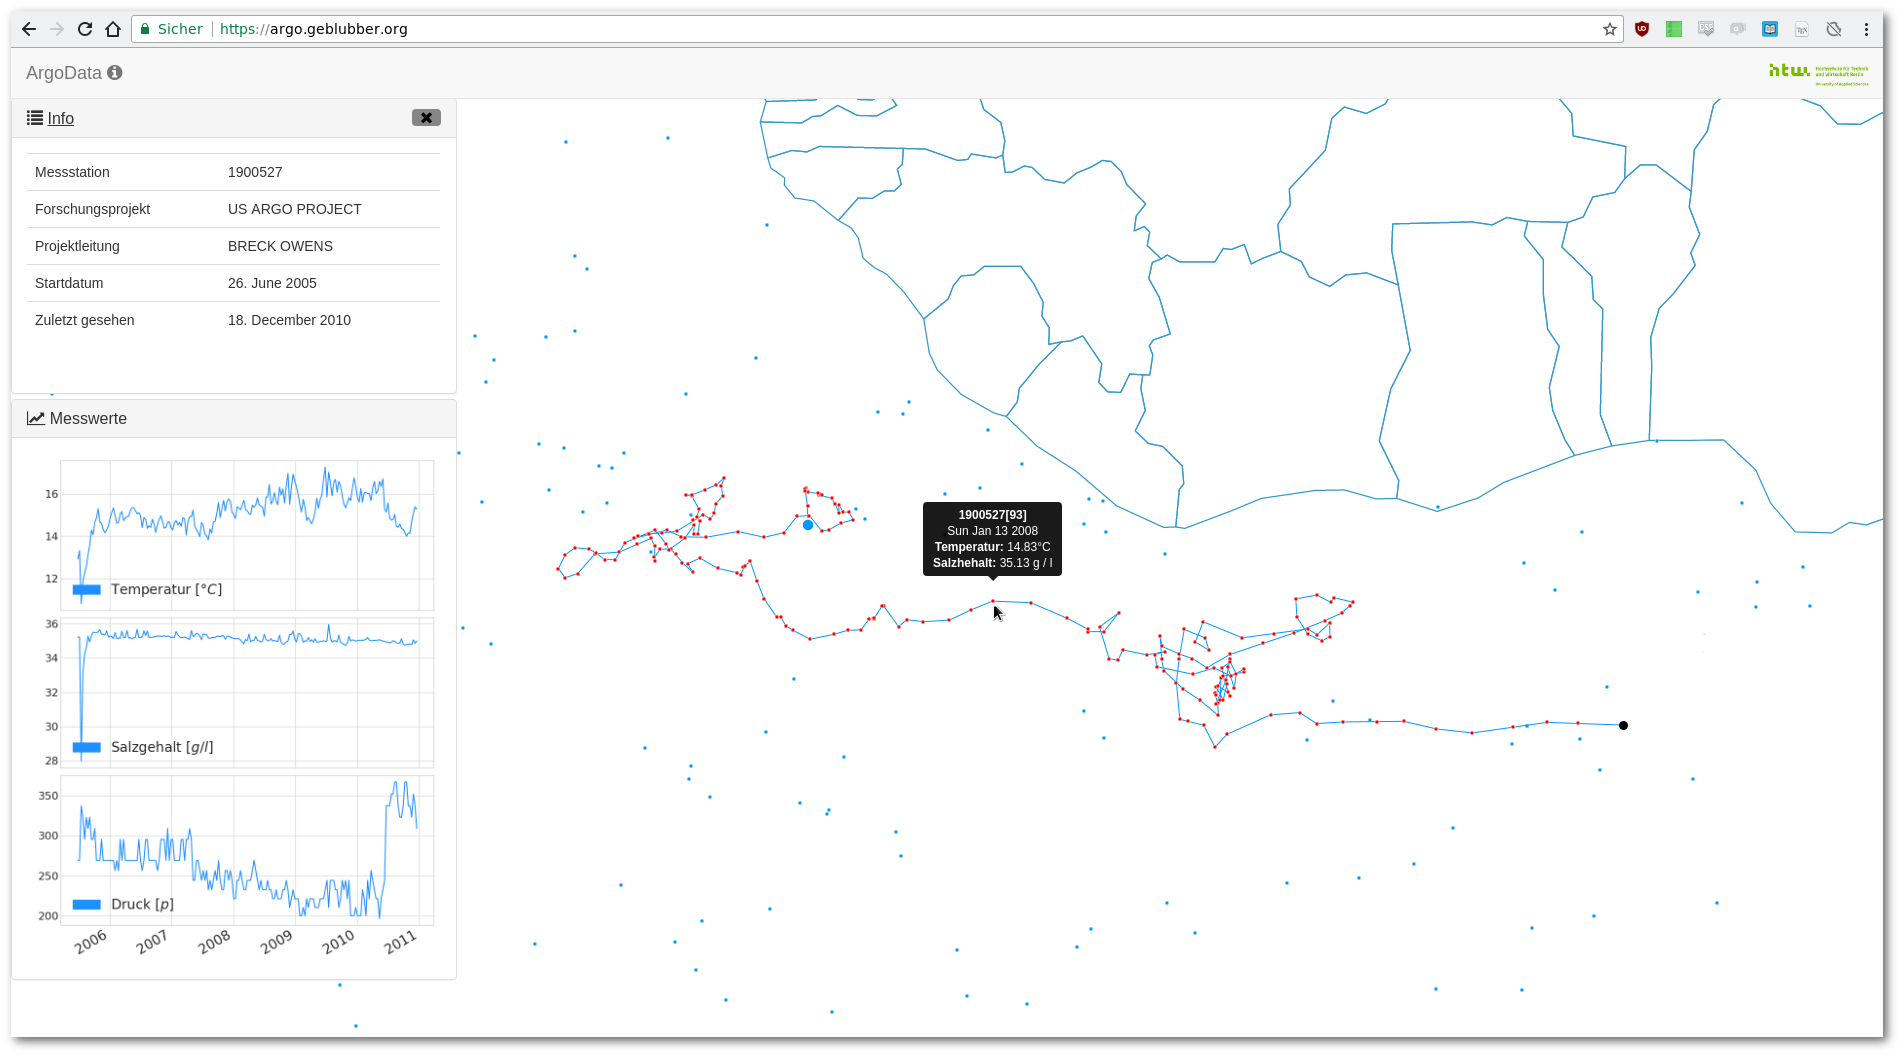
\includegraphics[width=\textwidth]{pix/argodata_complete.png}
 % argodata_complete.png: 1872x1026 px, 96dpi, 49.52x27.14 cm, bb=0 0 1404 769
 \caption{Die Webpräsenz von Argo-Data}
 \label{fig:argodataWeb}
\end{figure}




Damit endet diese Arbeit mit folgendem Zitat aus dem Buch "`\textit{Zen und die Kunst ein Motorrad zu warten}"' von Robert M. Pirsing:

\begin{quotation}
 Der echte Zug des Wissens ist nichts Statisches, das man anhalten und in Teile zerlegen kann. Er ist immer in Fahrt. Auf einem Gleis namens Qualität. Und die Lok und die 120 Güterwagen fahren nie woanders hin, als wo das Gleis der Qualität sie hinführt.
\end{quotation} 

